\documentclass[]{beamer}

\usefonttheme[onlymath]{serif}
\usepackage[]{graphicx}
\usepackage[]{minted}
\usepackage[]{enumitem}


\usetheme[]{Antibes}
\graphicspath{ {./images/} }
\title[]{Attention}
\author{HE Jiayou}

\AtBeginSection[]
{
    \begin{frame}
        \frametitle{Table of Contents}
        \tableofcontents[currentsection]
    \end{frame}
}

\AtBeginSubsection[]
{
    \begin{frame}
        \frametitle{Table of Contents}
        \tableofcontents[currentsection]
    \end{frame}
}

\AtBeginSubsubsection[]
{
    \begin{frame}
        \frametitle{Table of Contents}
        \tableofcontents[currentsection]
    \end{frame}
}

\begin{document}

\frame{\titlepage}

\begin{frame}
    \frametitle{Table of Contents}
    \tableofcontents
\end{frame}

\begin{frame}
    \frametitle{Notations}
    \begin{itemize}
        \item $n$: Batchsize
        \item $d$: Dimension of input
        \item $h$: Dimension of hidden state
        \item $q$: Dimension of answer
    \end{itemize}
\end{frame}

\section{RNN}
\begin{frame}
    \frametitle{RNN}
    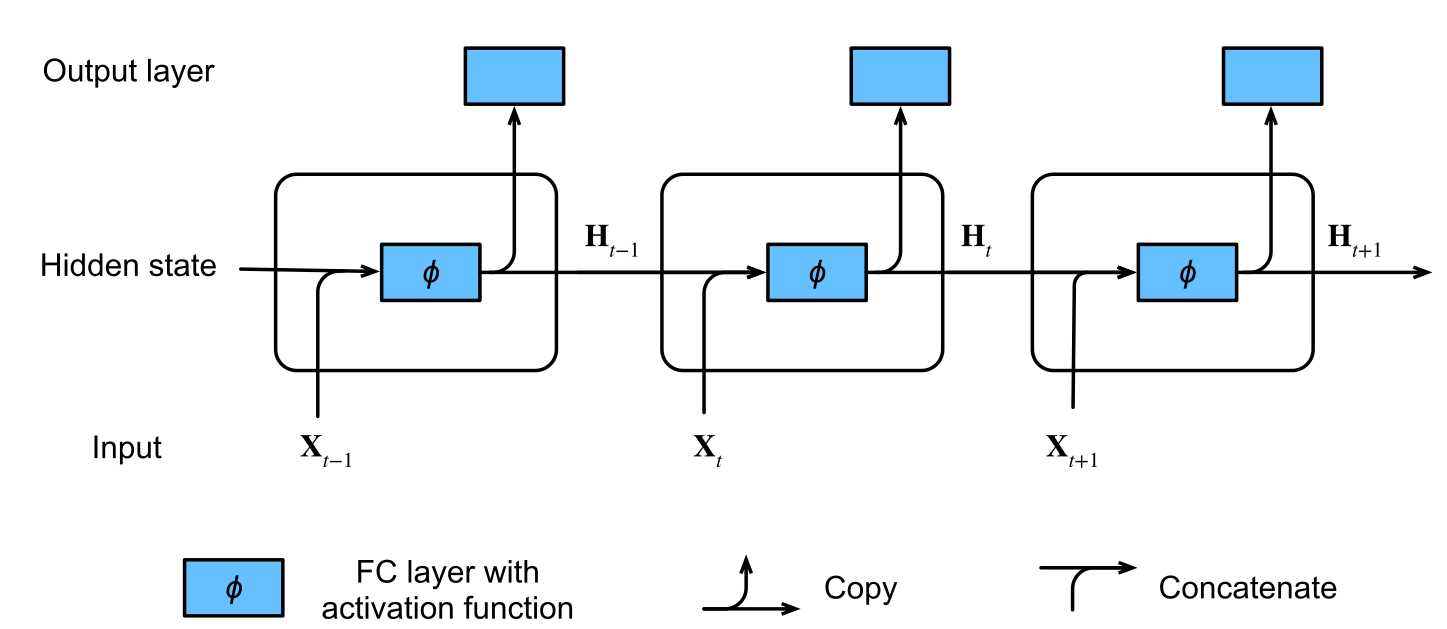
\includegraphics[scale = 0.2]{RNN.png}
    \begin{align*}
        H_t &= \phi\bigl(X_t W_{xh} + H_{t-1}W_{hh} + b_h\bigr) \\
        O_t &= H_t W_{hq} + b_q
    \end{align*}
\end{frame}

\subsection{GRU}
\begin{frame}
    \frametitle{GRU\: Gated Recurrent Unit}
    \begin{align*}
        R_t &= \sigma\bigl(X_t W_{xr} + H_{t-1}W_{hr} + b_r\bigr) \\
        Z_t &= \sigma\bigl(X_t W_{xz} + H_{t-1}W_{hz} + b_z\bigr) \\
        \tilde{H_t} &= \tanh \bigl(X_t W_{xh} + (R_t \odot H_{t-1})W_{hh} + b_h\bigr) \\
        H_t &= Z_t \odot H_{t-1} + (1-Z_t) \odot \tilde{H_t} 
    \end{align*}
    Being as an encoder.
\end{frame}

\subsection{LSTM}
\begin{frame}
    \frametitle{LSTM}
    Similar to GRU
    \begin{align*}
        I_t &= \sigma\bigl(X_t W_{xi} + H_{t-1}W_{hi} + b_i\bigr) \\
        F_t &= \sigma\bigl(X_t W_{xf} + H_{t-1} W_{hf} + b_f\bigr) \\
        O_t &= \sigma\bigl(X_t W_{xo} + H_{t-1} W_{ho} + b_o\bigr) \\
        \tilde{C_t} &= \tanh \bigl(X_t W_{xc} + H_{t-1}W_{hc} + b_c\bigr) \\
        C_t &= F_t \odot C_{t-1} + I_t \odot \tilde{C_t} \\
        H_t &= O_t \odot \tanh(C_t)
    \end{align*}
\end{frame}

\subsection{Encoder-Decoder}
\begin{frame}
    \frametitle{Encoder-Decoder}
\end{frame}

\section{Attention Prompt}
\begin{frame}
    \frametitle{Attention Prompt}
\end{frame}


\section{Transformer}
\begin{frame}
    \frametitle{Transformer}
\end{frame}

\subsection{architecture}
\begin{frame}
    \frametitle{architecture}
\end{frame}

\subsection{Attention}
\begin{frame}
    \frametitle{Attention}
\end{frame}

\subsubsection{Scoring Function}
\begin{frame}
    \frametitle{Scoring Function}
\end{frame}

\subsubsection{Multi-Head Attention}
\begin{frame}
    \frametitle{Multi-Head Attention}
\end{frame}

\subsubsection{Self-Attention}
\begin{frame}
    \frametitle{Self-Attention}
\end{frame}



\subsection{Positional Encoding}
\begin{frame}
    \frametitle{Positional Encoding}
\end{frame}

\subsection{Residual Connection \& Layer Normalization}
\begin{frame}
    \frametitle{Residual Connection \& Layer Normalization}
\end{frame}

\section{Medical-Related}
\begin{frame}
    \frametitle{Medical-Related}
\end{frame}

\subsection{Attention UNet}
\begin{frame}
    \frametitle{Attention UNet}
\end{frame}

\subsection{Multi-scale Self-guided Attention}
\begin{frame}
    \frametitle{Multi-scale Self-guided Attention}
\end{frame}

\end{document}